\smartsection{REST API \& Swagger}
\label{sec:rest-api}

\smartsubsection{Overview}

This section covers the assignment's Part~2 requirements (25 points): a
REST API exposing the system's live state and control surface, with
Swagger documentation. Per the assignment's explicit exception, all core
logic --- reading telemetry, dispatching commands, maintaining history ---
remains in C; a thin FastAPI layer adds only typed schemas and interactive
documentation on top, with zero business logic of its own.

\begin{lstlisting}[style=pythonstyle_bright_2026, caption={\texttt{gateway/main.py} --- the gateway's own docstring states its constraint plainly.}, label={code:gateway-constraint}]
"""
gateway/main.py -- Smart Surveillance System, Step 4 (REST API + Swagger)

THIN LAYER ONLY. Every endpoint here is a straight proxy to the C server
(see ../src/api_router.c) -- this file adds request/response typing for
Swagger UI and nothing else. No business logic, no data transformation,
no state.
"""
\end{lstlisting}

\smartsubsection{API Surface}

Beyond the five endpoints the assignment requires, two more were added

(\texttt{/api/v1/history/summary} and \texttt{/api/v1/services*}) since
they turned out to be useful for exercising and debugging the running
system during development, and cost little given the routing
infrastructure already existed.

\begin{table}[H]
\centering
\caption{Registered REST endpoints (\texttt{api\_router.c}).}
\label{tab:api-endpoints}
\resizebox{\textwidth}{!}{%
\begin{tabular}{lll}
\toprule
\textbf{Method} & \textbf{Path} & \textbf{Purpose} \\
\midrule
GET & \texttt{/api/v1/stream} & MJPEG live video (required) \\
GET & \texttt{/api/v1/frame.jpg} & Single current JPEG snapshot \\
GET & \texttt{/api/v1/persons} & Current person count + timestamp (required) \\
GET & \texttt{/api/v1/telemetry} & CPU temp, free memory, CPU load \% --- read directly in C (required) \\
POST & \texttt{/api/v1/command} & Extensible command dispatch, e.g.\ \texttt{\{"cmd": "reboot"\}} (required) \\
GET & \texttt{/api/v1/history} & Last 5 detection records (required) \\
GET & \texttt{/api/v1/history/summary} & Aggregate stats over the stored history (extension) \\
GET & \texttt{/api/v1/services} & Status of all systemd-managed services (extension) \\
POST & \texttt{/api/v1/services/\{name\}/restart} & Restart a named service (extension) \\
GET & \texttt{/api/v1/services/\{name\}/logs?lines=N} & Tail a service's journal (extension) \\
\bottomrule
\end{tabular}
}
\end{table}

\smartsubsubsection{Extensible Command Dispatch}

The assignment requires \texttt{/api/v1/command} to be "designed so new
commands can be added later without a rewrite." This is implemented as a
small table of command descriptors, each carrying its own
\texttt{dangerous} flag:

\begin{lstlisting}[style=cstyle_bright_2026, caption={Command table entry --- adding a new command is a one-line addition here, not a change to the dispatch logic.}, label={code:command-table}]
int dangerous; /* if 1, requires cfg->allow_dangerous_commands = true */
...
if (COMMANDS[i].dangerous && !cfg->allow_dangerous_commands) {
    /* refuse with a clear "marked dangerous" message */
}
\end{lstlisting}

Commands such as \texttt{reboot} and \texttt{shutdown} are marked
dangerous and refused by default; \texttt{allow\_dangerous\_commands} must
be explicitly set to \texttt{true} in \texttt{server.conf} before they will
actually execute, which keeps the default deployment safe from an
accidental (or malicious) reboot request while still satisfying the
"executable reboot command" requirement when deliberately enabled.

\smartsubsubsection{History (Last 5 Records)}

\texttt{history\_log.c} implements a fixed-size circular buffer
(\texttt{HISTORY\_SLOTS = 5}) rather than an unbounded log, satisfying the
"last 5 detection records" requirement directly at the data-structure
level rather than by truncating a query result.

\smartsubsection{Live Demonstration}

Figure~\ref{fig:api-requests} walks through the API surface end-to-end
against the deployed board: person count, full history, the history
summary, a harmless \texttt{noop} command exercising the dispatch
pipeline, a JPEG snapshot download, the services list/restart/logs
endpoints (including a live capture of \texttt{surveillance-imgproc}'s
retry logging from Section~\ref{sec:image-processing}), a full MJPEG
stream capture, and finally the dangerous-command safety switch correctly
refusing both \texttt{reboot} and \texttt{shutdown} while
\texttt{allow\_dangerous\_commands} is left at its default (\texttt{false}).

\begin{figure}[H]
\centering
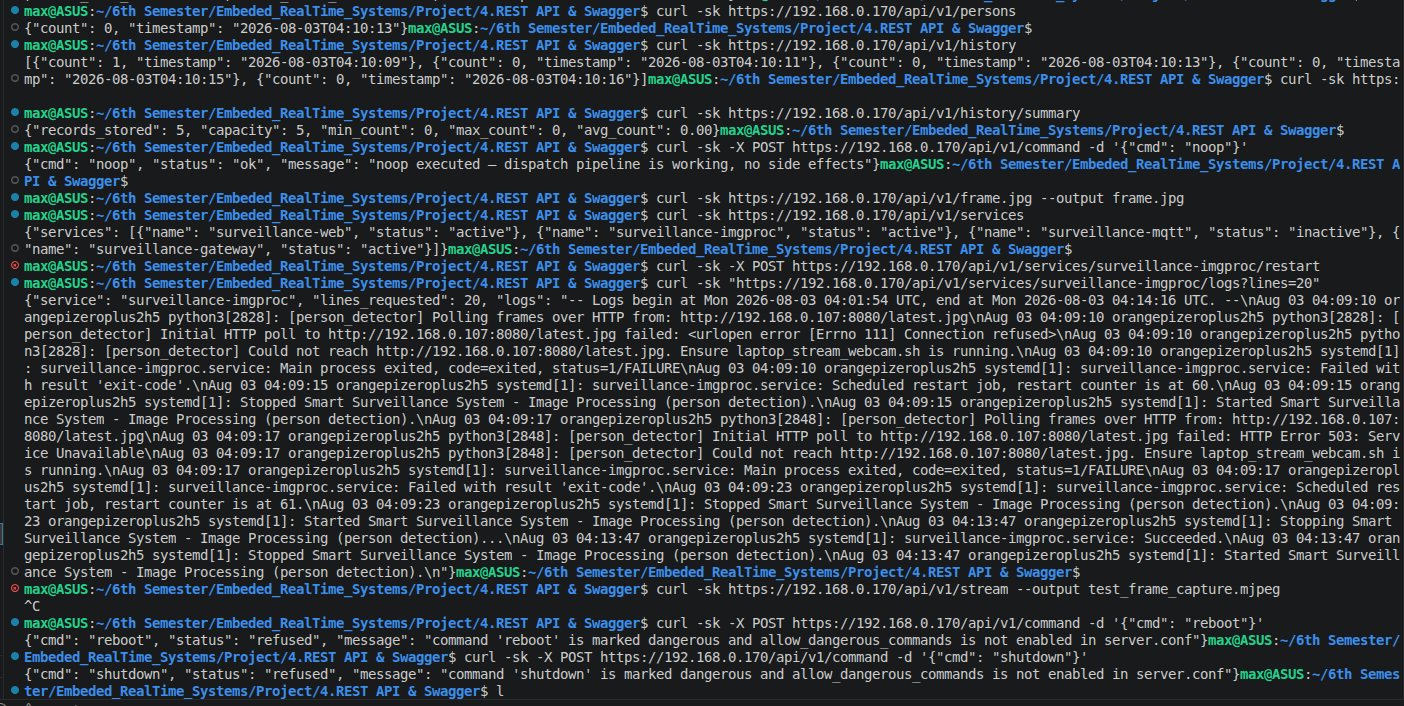
\includegraphics[width=0.95\textwidth]{../../4.REST API & Swagger/results/fig/api-requests.png}
\caption{End-to-end \texttt{curl} walkthrough of every registered endpoint against the live board.}\label{fig:api-requests}
\end{figure}

\smartsubsubsection{Verifying the Dangerous-Command Gate Actually Executes}

To confirm the refusal above is a genuine safety gate and not merely
cosmetic, \texttt{allow\_dangerous\_commands} was flipped to \texttt{true}
in \texttt{server.conf} and the reboot command was re-issued.

\begin{figure}[H]
\centering
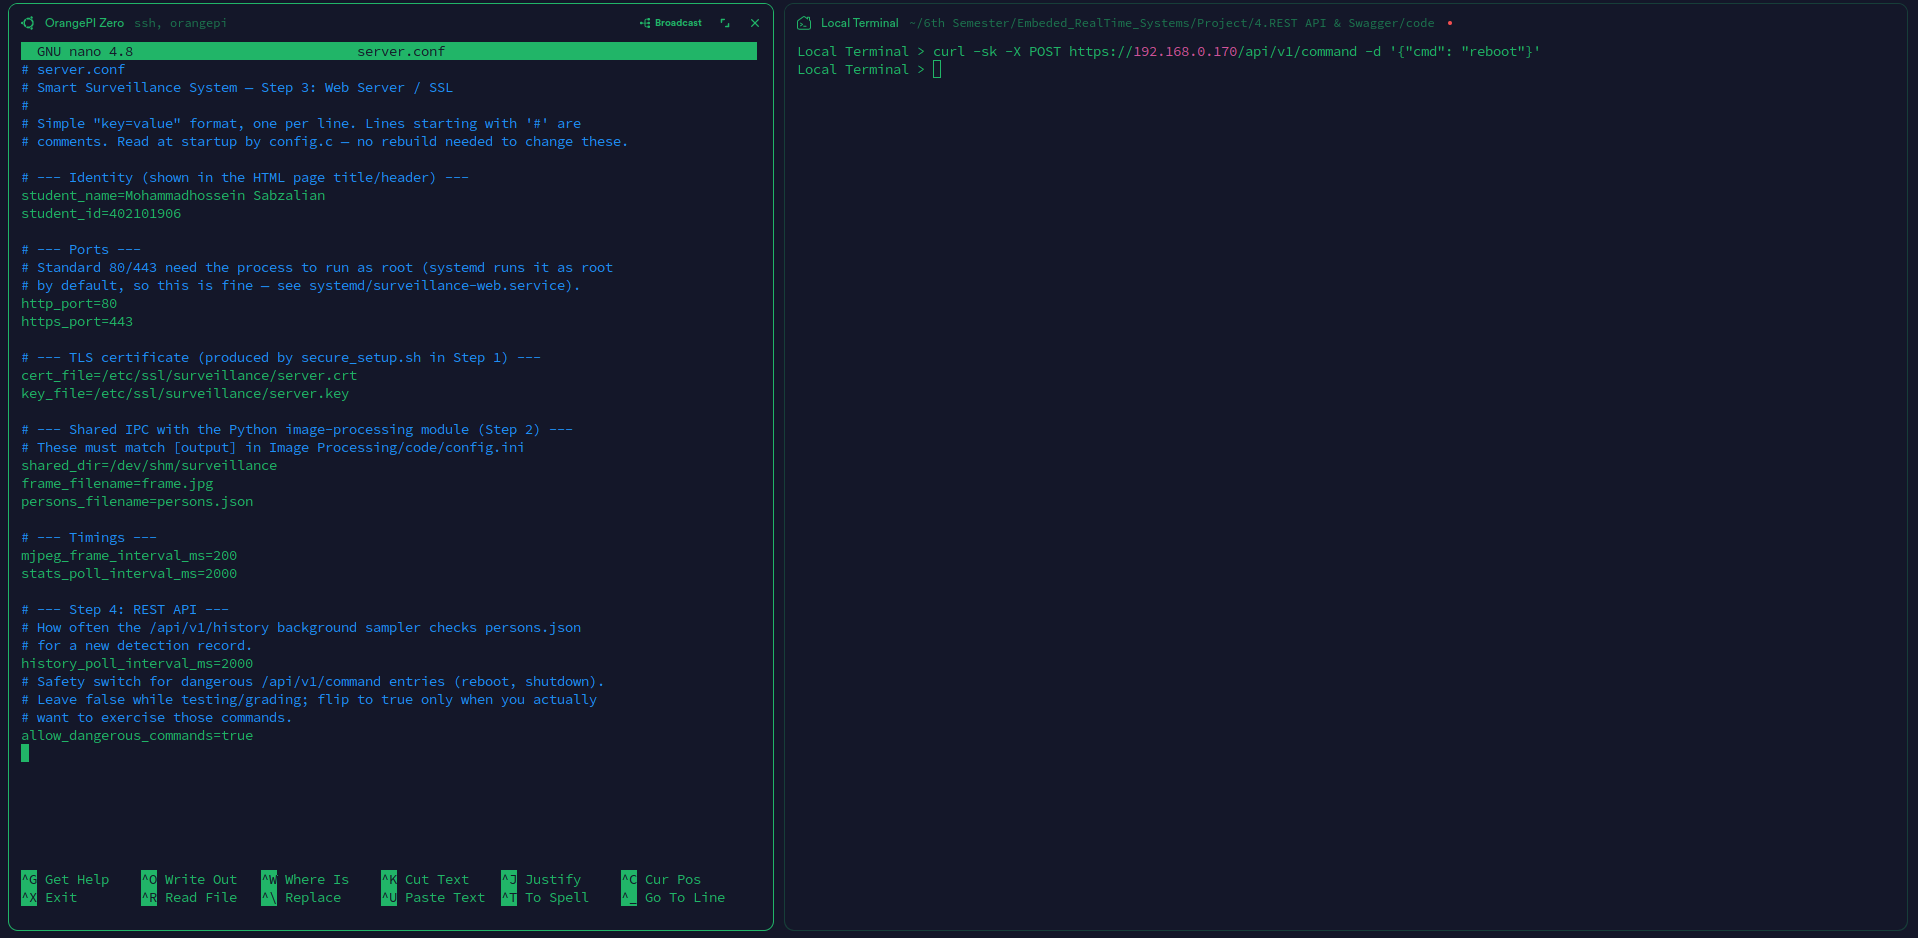
\includegraphics[width=0.95\textwidth]{../../4.REST API & Swagger/results/fig/api-reboot-allowed-test-config.png}
\caption{\texttt{server.conf} with \texttt{allow\_dangerous\_commands=true}, and the reboot request queued in a separate terminal.}\label{fig:reboot-config}
\end{figure}

\begin{figure}[H]
\centering
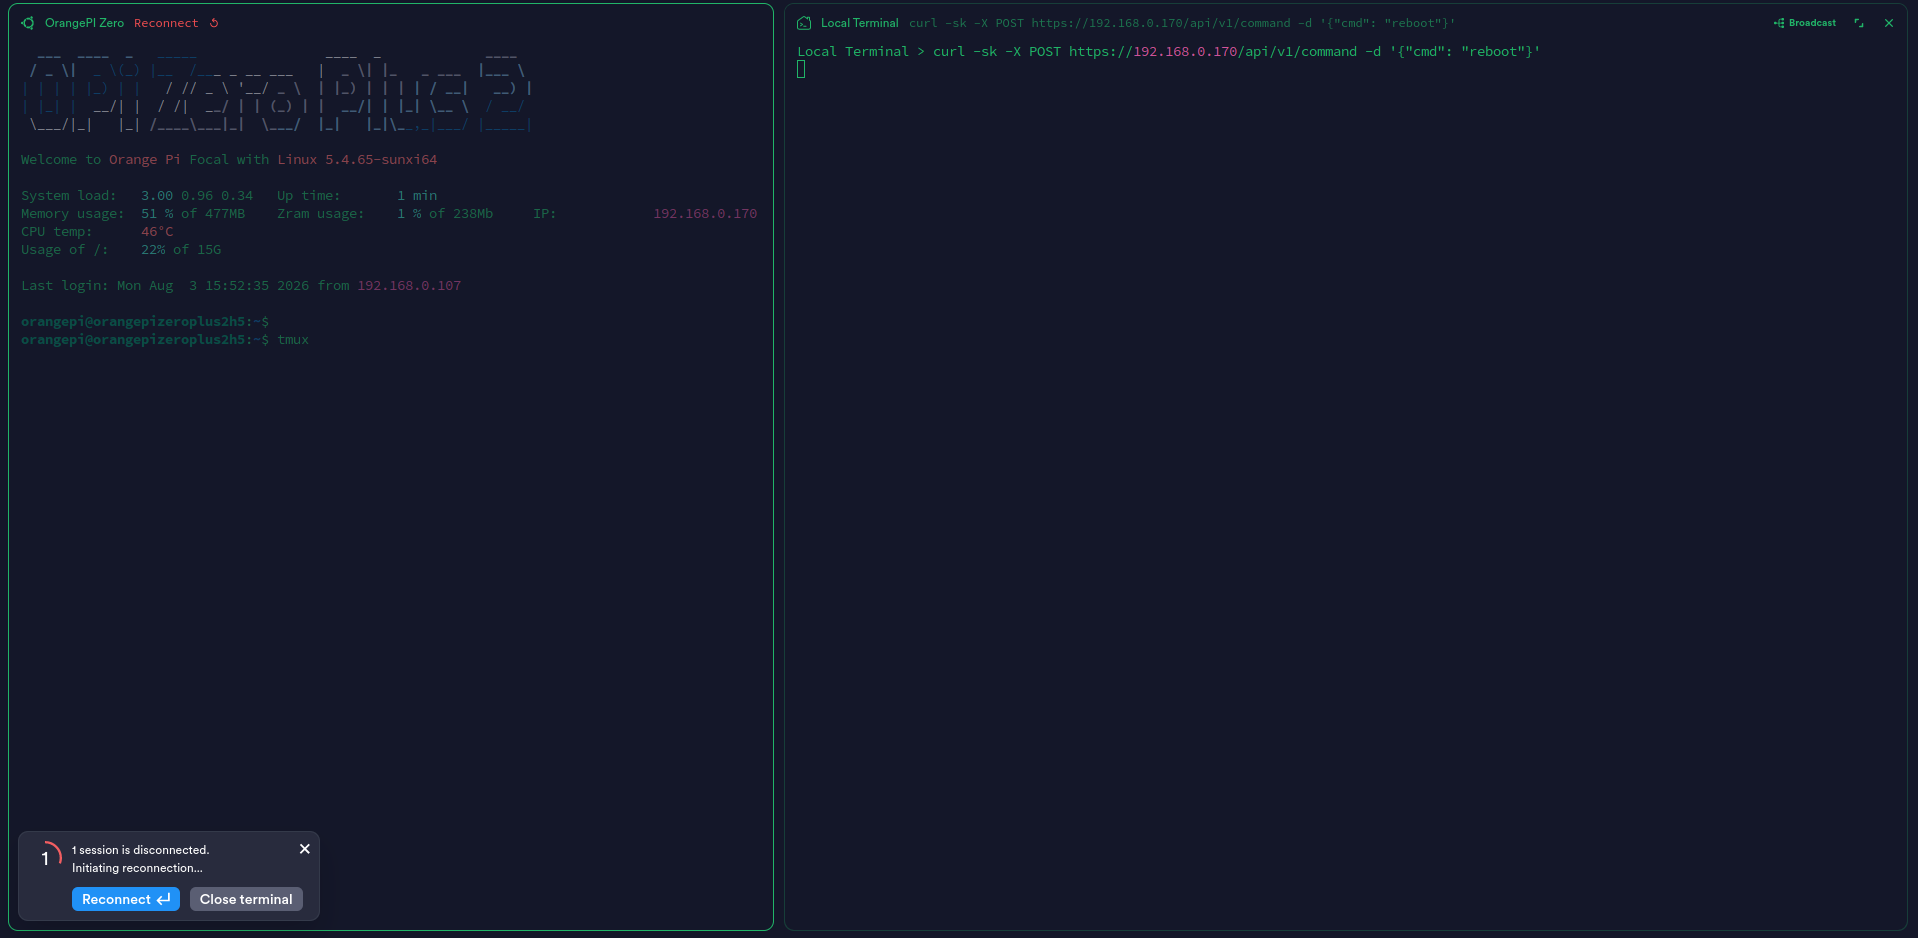
\includegraphics[width=0.95\textwidth]{../../4.REST API & Swagger/results/fig/api-reboot-allowed-test-during.png}
\caption{The board's SSH session drops immediately after the reboot command is issued, confirming a genuine reboot rather than a simulated response.}\label{fig:reboot-during}
\end{figure}

\smartsubsection{Swagger UI}

The FastAPI gateway exposes interactive documentation at \texttt{/docs}
for every endpoint in Table~\ref{tab:api-endpoints}, generated from the
Pydantic response models declared in \texttt{gateway/main.py} --- typing
only, with the C server remaining the source of truth for every value
returned.

\smartsubsection{Experiment 2-1: Temperature Under Three Conditions}
\label{sec:exp-2-1}

CPU temperature was sampled every 30\,s for 5 minutes under three
conditions using \texttt{exp2\_1\_temperature.py}: idle (nothing but the
C server running), streaming-only, and streaming with active person
detection.

\begin{figure}[H]
\centering
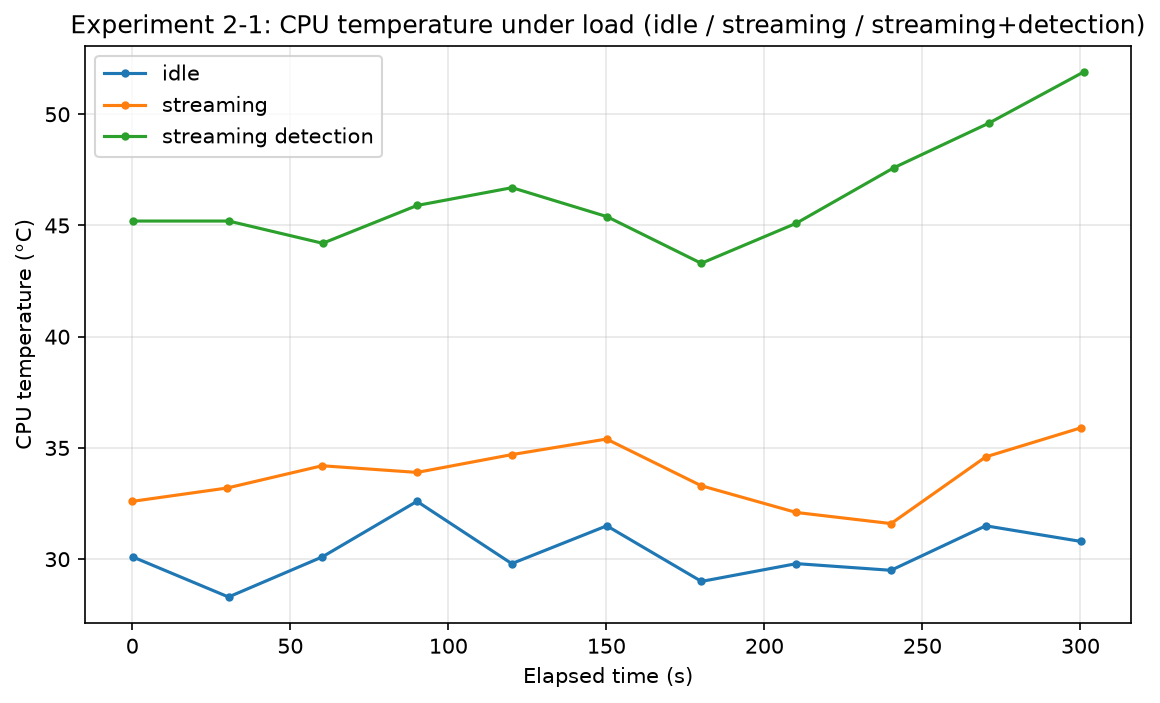
\includegraphics[width=0.8\textwidth]{../../4.REST API & Swagger/code/experiments/results/2-1/exp2_1_temperature.png}
\caption{CPU temperature over 5 minutes under idle, streaming-only, and streaming+detection conditions.}\label{fig:temp-3curve}
\end{figure}

\begin{table}[H]
\centering
\caption{Experiment 2-1 results: temperature by condition (11 samples each, 0 failed).}
\label{tab:temp-results}
\begin{tabular}{lccc}
\toprule
\textbf{Condition} & \textbf{Min (°C)} & \textbf{Max (°C)} & \textbf{Avg (°C)} \\
\midrule
Idle & 28.3 & 32.6 & 30.3 \\
Streaming only & 31.6 & 35.9 & 33.8 \\
Streaming + detection & 43.3 & \highlight{51.9} & 46.4 \\
\bottomrule
\end{tabular}
\end{table}

\begin{questionsection}{How does CPU temperature change across idle, streaming, and streaming+detection?}
The assignment asks for a graph comparing all three conditions and a
min/max summary table.
\end{questionsection}

\begin{answersection}{Analysis}
Idle and streaming-only both settle quickly and stay flat for the full
5 minutes, with streaming adding a modest $\sim$3.5\,°C over idle
(30.3\,°C~$\rightarrow$~33.8\,°C average) --- consistent with the
extra CPU cost of JPEG encoding and TLS in \texttt{https\_server.c}
alone. Streaming with detection enabled is a different story: it starts
$\sim$12.6\,°C above the streaming-only average and, unlike the other
two conditions, does not plateau --- it climbs steadily from 43.3\,°C
at $t{=}0$ to 51.9\,°C at $t{=}301$s, i.e.\ still rising at the end of
the 5-minute window. This suggests person-detection inference is
CPU-bound enough that 5 minutes is too short to see the board reach
thermal steady state under that load; a longer run would be needed to
confirm whether it plateaus below the SoC's throttling point or keeps
climbing.
\end{answersection}

\smartsubsection{Experiment 2-2: Memory Usage Over 5 Minutes of Streaming}
\label{sec:exp-2-2}

The web server process's memory usage was sampled every 5\,s over a
continuous 5-minute streaming session (61 samples) using
\texttt{exp2\_2\_memory.py}, with a linear trend fit to used memory over
time as a basic leak screen.

\begin{figure}[H]
\centering
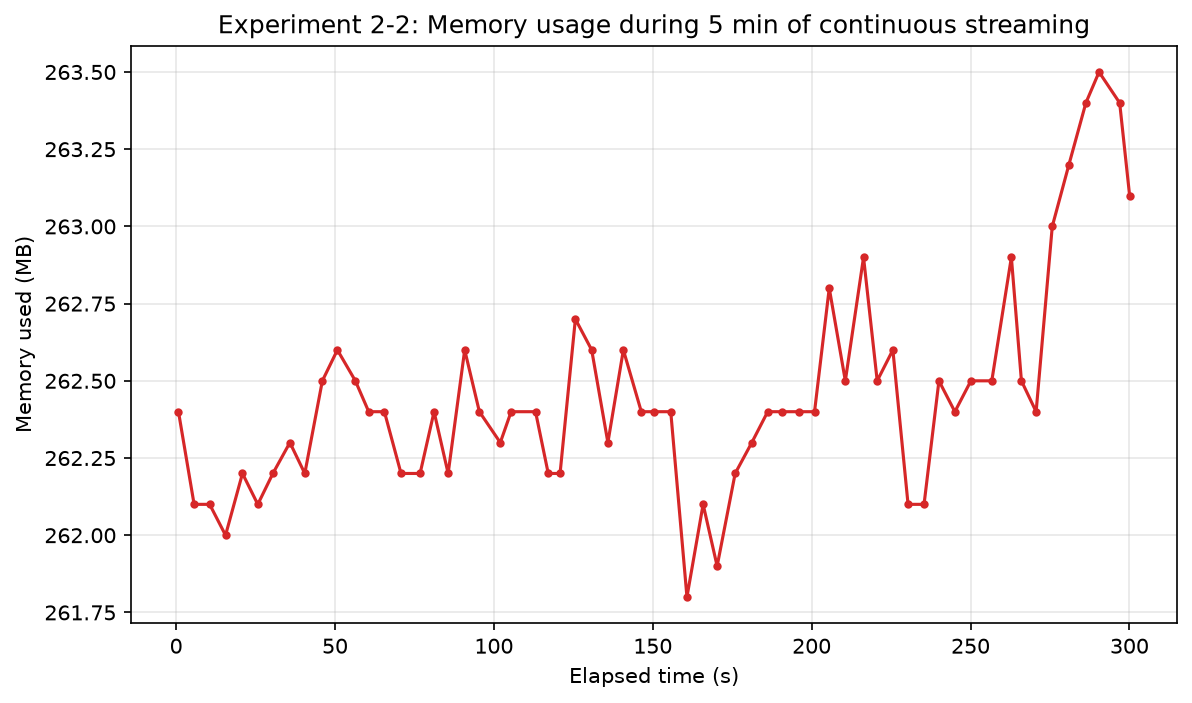
\includegraphics[width=0.8\textwidth]{../../4.REST API & Swagger/code/experiments/results/2-2/exp2_2_memory.png}
\caption{Memory used over 5 minutes of continuous MJPEG streaming.}\label{fig:memory-5min}
\end{figure}

\begin{table}[H]
\centering
\caption{Experiment 2-2 leak-screen results.}
\label{tab:memory-results}
\begin{tabular}{lc}
\toprule
\textbf{Metric} & \textbf{Value} \\
\midrule
First sample used & 262.4\,MB \\
Last sample used & 263.1\,MB \\
Peak used & 263.5\,MB \\
Net change & +0.7\,MB \\
Linear trend slope & +0.137\,MB/min \\
\bottomrule
\end{tabular}
\end{table}

\begin{questionsection}{Does memory usage grow over a sustained streaming session?}
The assignment asks for a graph of memory usage over the 5-minute
window and a basic leak analysis.
\end{questionsection}

\begin{answersection}{Analysis}
Used memory stayed within a $\sim$1.4\,MB band across the full 5
minutes (net change +0.7\,MB, peak 263.5\,MB), and the fitted trend of
+0.137\,MB/min extrapolates to well under 10\,MB/hour --- \stable{no
meaningful upward trend}, consistent with no leak over this window. As
the script's own output notes, this slope is a screening heuristic
over a short window, not proof of leak-free operation; the honest
conclusion is "no leak detected in 5 minutes of streaming," not "leak
free," and a 30--60 minute run would be the appropriate follow-up if
this were headed to production rather than coursework.
\end{answersection}

\smartsubsection{Experiment 2-3: 50 Concurrent Requests}
\label{sec:exp-2-3}

Fifty concurrent requests were fired at \texttt{/api/v1/telemetry} using
\texttt{exp2\_3\_concurrency.py}, with system telemetry sampled
immediately before the burst, immediately after, and again ten seconds
later once the system had settled.

\begin{figure}[H]
\centering
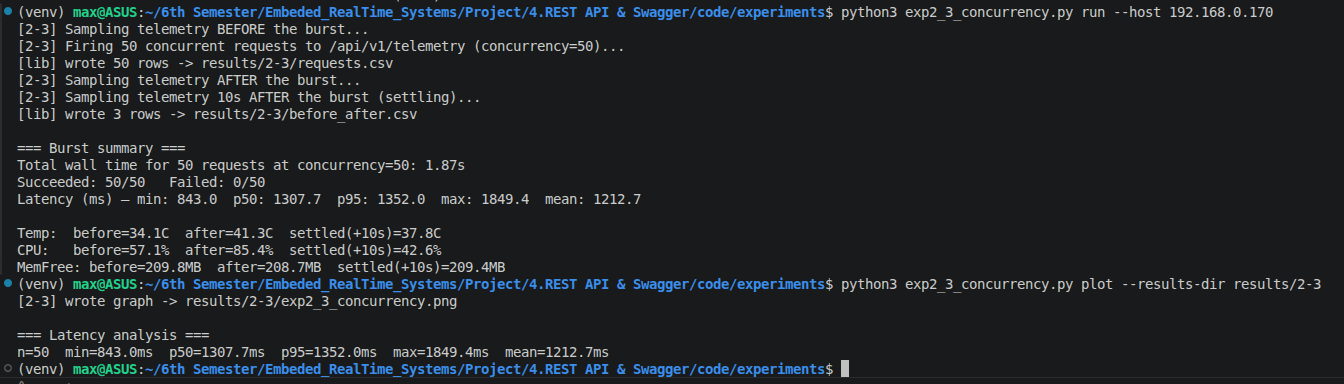
\includegraphics[width=0.95\textwidth]{../../4.REST API & Swagger/results/fig/50-concurrency-test.png}
\caption{50 concurrent requests to \texttt{/api/v1/telemetry}: full run output including before/after/settled telemetry and latency percentiles.}\label{fig:concurrency-50}
\end{figure}

\begin{table}[H]
\centering
\caption{Experiment 2-3 results: 50 concurrent requests to \texttt{/api/v1/telemetry}.}
\label{tab:concurrency-results}
\begin{tabular}{lc}
\toprule
\textbf{Metric} & \textbf{Value} \\
\midrule
Requests succeeded / failed & \stable{50 / 50} succeeded, 0 failed \\
Total wall time for the burst & 1.87\,s \\
Latency --- min & 843.0\,ms \\
Latency --- p50 (median) & 1307.7\,ms \\
Latency --- p95 & 1352.0\,ms \\
Latency --- max & \highlight{1849.4\,ms} \\
Latency --- mean & 1212.7\,ms \\
CPU temperature --- before / after / settled (+10s) & 34.1\,°C / 41.3\,°C / 37.8\,°C \\
CPU usage --- before / after / settled (+10s) & 57.1\% / \alert{85.4\%} / 42.6\% \\
Free memory --- before / after / settled (+10s) & 209.8\,MB / 208.7\,MB / 209.4\,MB \\
\bottomrule
\end{tabular}
\end{table}

\begin{questionsection}{What happens to latency and system load under 50 concurrent requests?}
The assignment asks for a graph of the resulting temperature/CPU/memory
changes and an analysis of the response-latency increase.
\end{questionsection}

\begin{answersection}{Analysis}
All 50 requests succeeded with zero failures, and the entire burst
completed in under two seconds --- the one-thread-per-connection model in
\texttt{https\_server.c} (Section~\ref{sec:web-server}) handled the load
without dropping a single connection. The cost is visible in tail latency
rather than failures: the gap between the median (1307.7\,ms) and the
maximum (1849.4\,ms) shows the later-arriving requests in the burst
queuing behind earlier ones as fifty simultaneous TLS handshakes and
\texttt{/proc} reads contend for the board's four Cortex-A53 cores. CPU
usage jumped from a baseline 57.1\% to 85.4\% during the burst, and
temperature rose measurably (34.1\,°C~$\rightarrow$~41.3\,°C) despite the
burst lasting under two seconds, showing the instantaneous load spike is
real even though it is brief. Notably, all three metrics --- temperature,
CPU, and free memory --- returned close to their pre-burst baselines
within the 10-second settling window, indicating no resource leak or
lingering thread pileup from the concurrent load.
\end{answersection}

\smartsubsection{Experiment 2-4: Network Disconnect / Reconnect}
\label{sec:exp-2-4}

\texttt{exp2\_4\_network\_recovery.py} watched the MJPEG stream client
and polled the server's health while the network link was cut mid-stream
and restored, and captured \texttt{journalctl} output for
\texttt{surveillance-web} over the same window to check whether the
service itself needed to restart.

\begin{figure}[H]
\centering
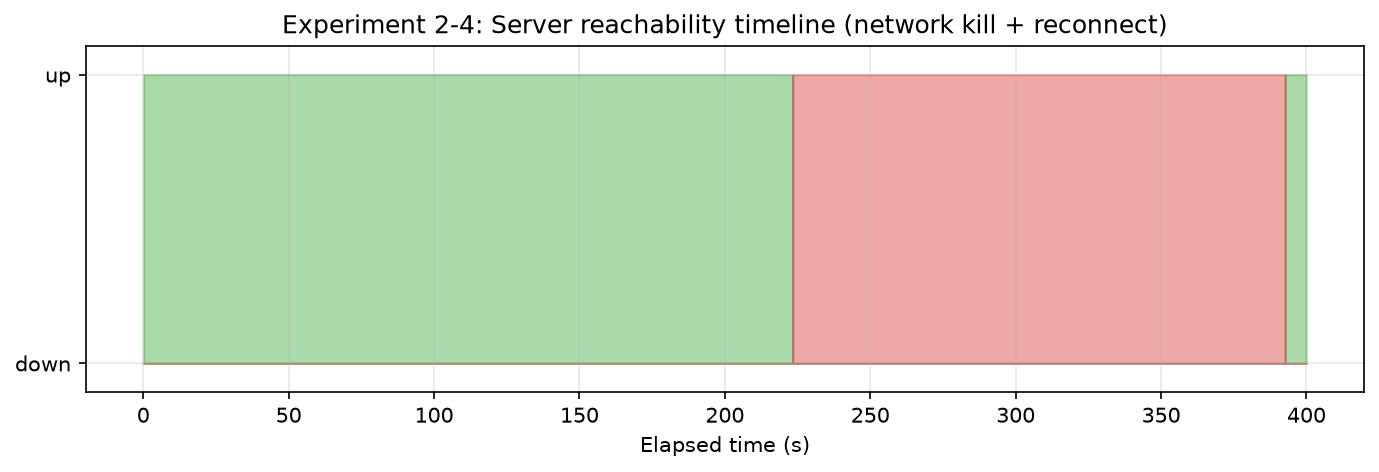
\includegraphics[width=0.8\textwidth]{../../4.REST API & Swagger/code/experiments/results/2-4/exp2_4_recovery_timeline.png}
\caption{Client-observed stream health and reconnect timeline across the network outage.}\label{fig:network-recovery}
\end{figure}

\begin{table}[H]
\centering
\caption{Experiment 2-4 results: network disconnect/reconnect.}
\label{tab:network-results}
\begin{tabular}{lc}
\toprule
\textbf{Metric} & \textbf{Value} \\
\midrule
Stream connected (initial) & $t{=}0.06$\,s \\
Connection lost (stream client) & $t{=}228.9$\,s \\
Connection lost (health monitor, first timeout) & $t{=}223.3$\,s \\
Reconnect attempts during outage & 52 (retried every $\sim$3\,s) \\
Stream reconnected & $t{=}391.8$\,s \\
Health monitor confirmed \texttt{up} again & $t{=}392.7$\,s, latency back to 62.5\,ms \\
Total observed outage & \highlight{$\sim$163--169\,s ($\sim$2.7--2.8\,min)} \\
\texttt{journalctl} entries for \texttt{surveillance-web} during outage & \stable{none} \\
\bottomrule
\end{tabular}
\end{table}

\begin{questionsection}{What happens to the stream and the server when the network drops mid-session, and does the service need to restart?}
The assignment asks for the client-observed stream behavior, the
server-side log behavior, and a characterization of the recovery.
\end{questionsection}

\begin{answersection}{Analysis}
Once the link was cut, the stream client detected the loss within
$\sim$5.6\,s (via a read timeout) and immediately began retrying every
$\sim$3\,s, logging 52 consecutive \texttt{ConnectionError}/
\texttt{ConnectTimeout} attempts before the network came back --- the
retry loop never gave up or backed off further, it just kept trying at
a fixed interval for the whole $\sim$2.7-minute outage. As soon as the
link was physically restored, the very next attempt succeeded
(reconnected at $t{=}391.8$\,s) and latency dropped straight back to its
pre-outage baseline ($\sim$50--90\,ms) with no warm-up period, after
which streaming continued to completion. Critically,
\texttt{journalctl} shows \emph{zero} log entries for
\texttt{surveillance-web} across the entire outage window --- the
server process never crashed, never restarted, and never even logged
the dropped connection; from the service's point of view nothing
happened. This confirms the recovery is entirely client-driven: the
systemd service does not need to restart after a network blip, because
the C server was never the thing that went away.
\end{answersection}

\smartsubsection{Section Summary}

\begin{table}[H]
\centering
\caption{REST API \& Swagger deliverables completed in this section.}
\label{tab:api-summary}
\begin{tabular}{ll}
\toprule
\textbf{Item} & \textbf{Status} \\
\midrule
\texttt{GET /api/v1/stream} & Complete \\
\texttt{GET /api/v1/persons} & Complete \\
\texttt{GET /api/v1/telemetry} (direct C reads, no shell-out) & Complete \\
\texttt{POST /api/v1/command} (extensible, safety-gated) & Complete \\
\texttt{GET /api/v1/history} (5-slot circular buffer) & Complete \\
Swagger UI (FastAPI thin gateway) & Complete \\
Exp.\ 2-1 (temperature, 3 conditions) & Complete --- Table~\ref{tab:temp-results} \\
Exp.\ 2-2 (memory over 5 min) & Complete --- Table~\ref{tab:memory-results} \\
Exp.\ 2-3 (50 concurrent requests) & Complete --- Table~\ref{tab:concurrency-results} \\
Exp.\ 2-4 (network disconnect/reconnect) & Complete --- Table~\ref{tab:network-results} \\
\bottomrule
\end{tabular}
\end{table}
